% Options for packages loaded elsewhere
\PassOptionsToPackage{unicode}{hyperref}
\PassOptionsToPackage{hyphens}{url}
\PassOptionsToPackage{dvipsnames,svgnames,x11names}{xcolor}
%
\documentclass[
  ignorenonframetext,
]{beamer}
\usepackage{pgfpages}
\setbeamertemplate{caption}[numbered]
\setbeamertemplate{caption label separator}{: }
\setbeamercolor{caption name}{fg=normal text.fg}
\beamertemplatenavigationsymbolsempty
% Prevent slide breaks in the middle of a paragraph
\widowpenalties 1 10000
\raggedbottom
\setbeamertemplate{part page}{
  \centering
  \begin{beamercolorbox}[sep=16pt,center]{part title}
    \usebeamerfont{part title}\insertpart\par
  \end{beamercolorbox}
}
\setbeamertemplate{section page}{
  \centering
  \begin{beamercolorbox}[sep=12pt,center]{part title}
    \usebeamerfont{section title}\insertsection\par
  \end{beamercolorbox}
}
\setbeamertemplate{subsection page}{
  \centering
  \begin{beamercolorbox}[sep=8pt,center]{part title}
    \usebeamerfont{subsection title}\insertsubsection\par
  \end{beamercolorbox}
}
\AtBeginPart{
  \frame{\partpage}
}
\AtBeginSection{
  \ifbibliography
  \else
    \frame{\sectionpage}
  \fi
}
\AtBeginSubsection{
  \frame{\subsectionpage}
}
\usepackage{amsmath,amssymb}
\usepackage{lmodern}
\usepackage{iftex}
\ifPDFTeX
  \usepackage[T1]{fontenc}
  \usepackage[utf8]{inputenc}
  \usepackage{textcomp} % provide euro and other symbols
\else % if luatex or xetex
  \usepackage{unicode-math}
  \defaultfontfeatures{Scale=MatchLowercase}
  \defaultfontfeatures[\rmfamily]{Ligatures=TeX,Scale=1}
\fi
% Use upquote if available, for straight quotes in verbatim environments
\IfFileExists{upquote.sty}{\usepackage{upquote}}{}
\IfFileExists{microtype.sty}{% use microtype if available
  \usepackage[]{microtype}
  \UseMicrotypeSet[protrusion]{basicmath} % disable protrusion for tt fonts
}{}
\makeatletter
\@ifundefined{KOMAClassName}{% if non-KOMA class
  \IfFileExists{parskip.sty}{%
    \usepackage{parskip}
  }{% else
    \setlength{\parindent}{0pt}
    \setlength{\parskip}{6pt plus 2pt minus 1pt}}
}{% if KOMA class
  \KOMAoptions{parskip=half}}
\makeatother
\usepackage{xcolor}
\newif\ifbibliography
\usepackage{graphicx}
\makeatletter
\def\maxwidth{\ifdim\Gin@nat@width>\linewidth\linewidth\else\Gin@nat@width\fi}
\def\maxheight{\ifdim\Gin@nat@height>\textheight\textheight\else\Gin@nat@height\fi}
\makeatother
% Scale images if necessary, so that they will not overflow the page
% margins by default, and it is still possible to overwrite the defaults
% using explicit options in \includegraphics[width, height, ...]{}
\setkeys{Gin}{width=\maxwidth,height=\maxheight,keepaspectratio}
% Set default figure placement to htbp
\makeatletter
\def\fps@figure{htbp}
\makeatother
\setlength{\emergencystretch}{3em} % prevent overfull lines
\providecommand{\tightlist}{%
  \setlength{\itemsep}{0pt}\setlength{\parskip}{0pt}}
\setcounter{secnumdepth}{-\maxdimen} % remove section numbering

\usepackage{textpos}
\setbeamertemplate{headline}{
  \begin{textblock*}{5cm}(10.2cm,0.2cm)
  
\includegraphics[width=2.2cm]{UniUrb-logo.png}
  \end{textblock*}}
  
  \definecolor{myblue}{HTML}{005997}
  \setbeamercolor{frametitle}{fg=myblue}
    \setbeamercolor{framesubtitle}{fg=myblue}
    \setbeamercolor{frametitle right}{fg=myblue}
  \setbeamercolor{titlelike}{fg=myblue}
    \setbeamercolor{title}{fg=myblue}
      \setbeamercolor{subtitle}{fg=myblue}
    \setbeamercolor{part title}{fg=myblue}
    \setbeamercolor{section title}{fg=myblue}
    \setbeamercolor{subsection title}{fg=myblue}
  \setbeamercolor{section name}{fg=myblue}
  \setbeamercolor{subsection name}{fg=myblue}
  \setbeamercolor{part name}{fg=myblue}
  \setbeamercolor{title in head/foot}{fg=myblue}
  \setbeamercolor{subtitle in head/foot}{fg=myblue}
  \setbeamercolor{block title}{fg=myblue}
  
  \setbeamercolor{bullet}{fg=myblue}
  \setbeamercolor{section in toc}{fg=myblue}
  \setbeamercolor{subsection in toc}{fg=myblue}
  \setbeamercolor{section in head/foot}{fg=myblue}
  \setbeamercolor{subsection in head/foot}{fg=myblue}
  
  
  \setbeamercolor{itemize item}{fg = myblue}
  \setbeamercolor{itemize subitem}{fg = myblue}
  \setbeamercolor{itemize subsubitem}{fg = myblue}
  \setbeamercolor{enumerate item}{fg = myblue}
  \setbeamercolor{enumerate subitem}{fg = myblue}
  \setbeamercolor{enumerate subsubitem}{fg = myblue}
  
 
  
\usepackage{etoolbox}
\AtBeginEnvironment{thebibliography}{\scriptsize}
\ifLuaTeX
  \usepackage{selnolig}  % disable illegal ligatures
\fi
\usepackage[round]{natbib}
\bibliographystyle{apalike}
\IfFileExists{bookmark.sty}{\usepackage{bookmark}}{\usepackage{hyperref}}
\IfFileExists{xurl.sty}{\usepackage{xurl}}{} % add URL line breaks if available
\urlstyle{same} % disable monospaced font for URLs
\hypersetup{
  pdftitle={Bibliometric Analysis of European Research on Digital Divide: An Exploration of the Corporate Landscape},
  pdfauthor={Luis Carlos Castillo},
  colorlinks=true,
  linkcolor={myblue},
  filecolor={Maroon},
  citecolor={Blue},
  urlcolor={Blue},
  pdfcreator={LaTeX via pandoc}}

\title{Bibliometric Analysis of European Research on Digital Divide: An
Exploration of the Corporate Landscape}
\author{Luis Carlos Castillo}
\date{16 May 2023}
\institute{University of Urbino\\
Ph.D.~Program in Global Studies}

\begin{document}
\frame{\titlepage}

\begin{frame}{Content I}
\protect\hypertarget{content-i}{}
\begin{enumerate}
\item
  Digital Divide Overview
\item
  Motivation
\item
  Objectives and Research Questions
\item
  Data
\item
  Bibliometric Analysis
\item
  Performance Analysis

  \begin{enumerate}
  \tightlist
  \item
    Publications Vs Citations
  \item
    Authors
  \item
    Articles
  \item
    Journals
  \item
    Affiliations/ Universities
  \item
    Countries
  \end{enumerate}
\end{enumerate}
\end{frame}

\begin{frame}{Content II}
\protect\hypertarget{content-ii}{}
\begin{enumerate}
\setcounter{enumi}{6}
\item
  Science Mapping

  \begin{enumerate}
  \tightlist
  \item
    Citations Analysis
  \item
    Similarity Measures

    \begin{enumerate}
    \tightlist
    \item
      Co-citations Analysis
    \item
      Bibliographic Coupling
    \item
      Co-word Analysis
    \end{enumerate}
  \end{enumerate}
\item
  Conclusions
\end{enumerate}
\end{frame}

\begin{frame}{1. The Digital Divide Overview I}
\protect\hypertarget{the-digital-divide-overview-i}{}
\begin{itemize}
\tightlist
\item
  The digital divide is also known as the digital gap, inequalities, or
  disparities.
\item
  The interaction with other existing gaps such as income, education,
  gender, age, and regional, among others \citep{ragnedda2017}.
\item
  The evolution of the concept has pointed out the phenomenon's
  complexity and the effects on the different layers of society and the
  economy \citep{vandijk2003, ragnedda2017, shakina2021}.
\end{itemize}
\end{frame}

\begin{frame}{1. The Digital Divide Overview II}
\protect\hypertarget{the-digital-divide-overview-ii}{}
\begin{itemize}
\tightlist
\item
  Waves of Research

  \begin{itemize}
  \item
    \textbf{The first wave:} Physical access to technology
    -\textgreater{} possession of computers and access to the internet
    \citep{norris2001, james2002, castells2003}.
  \item
    \textbf{The second wave:} Usage of digital technologies and skills
    \citep{hargittai2002b, vandijk2005b, vandijk2006c, vandeursen2011c}.
  \item
    The divide is not exclusively a matter of access or possession of
    technology. It encloses the ability to effectively search, access,
    and evaluate information using digital technologies.
  \end{itemize}
\end{itemize}
\end{frame}

\begin{frame}{1. The Digital Divide Overview III}
\protect\hypertarget{the-digital-divide-overview-iii}{}
\begin{itemize}
\tightlist
\item
  Waves of Research

  \begin{itemize}
  \item
    \textbf{The third wave:} expands upon the inequalities previously
    identified in the 1st and 2nd wave.
  \item
    Focuses on the benefits previously gained from access, skills, and
    usage of digital technologies.
  \item
    Emphasize on the ability to benefit from digital technologies in a
    data-driven market to improve personal and professional aspects
    \citep{ragnedda2017}.
  \item
    The disparities from the tangible outcomes gained from different
    forms of access and usage of digital technologies
    \citep{vandeursen2015}.
  \end{itemize}
\end{itemize}
\end{frame}

\begin{frame}{1. The digital divide overview VI}
\protect\hypertarget{the-digital-divide-overview-vi}{}
\begin{block}{The corporate landscape}
\protect\hypertarget{the-corporate-landscape}{}
\begin{itemize}
\tightlist
\item
  Digital revolution -\textgreater{} different aspects of daily
  activities -\textgreater{} how we conduct business.
\item
  Disparity in digital capabilities and resources among businesses
  \citep{shakina2021}.
\item
  The corporate digital divide is a topic that remains under-explored
  \citep{pejicbach2013, shakina2021}.
\item
  Understanding and addressing the divide, policymakers, and businesses
  owners can target their efforts to ensure inclusive digital
  transformation.
\end{itemize}
\end{block}
\end{frame}

\begin{frame}{2. Motivation}
\protect\hypertarget{motivation}{}
\begin{itemize}
\item
  Investigating the transformative effects of digital technologies on
  society and economy, while highlighting both opportunities and
  challenges.
\item
  Aligning with the Digital Europe program's vision by devising
  strategies to bridge the digital divide effectively.
\item
  Diversifying bibliometric research by extending its application beyond
  health sciences, computer science, and technology to understand the
  digital divide.
\item
  Harnessing the power of comprehensive data from three leading academic
  platforms to generate insightful and actionable findings on the
  digital divide.
\end{itemize}
\end{frame}

\begin{frame}{3. Objectives and Research Questions I}
\protect\hypertarget{objectives-and-research-questions-i}{}
\begin{block}{Objectives}
\protect\hypertarget{objectives}{}
\begin{itemize}
\item
  Understand the intellectual structure within the domain of the digital
  divide.
\item
  Examine the intellectual interactions, and thematic relationships of
  European research components.
\item
  Explore the corporate digital divide among the collected corpus and
  identify trends and patterns within the literature.
\end{itemize}
\end{block}
\end{frame}

\begin{frame}{3. Objectives and Research Questions II}
\protect\hypertarget{objectives-and-research-questions-ii}{}
\begin{block}{Research Questions}
\protect\hypertarget{research-questions}{}
\begin{itemize}
\item
  Q1: How have the main trends, focus shifts, and key themes in European
  research on the digital divide evolved over time, and how do they
  reflect the current state of knowledge in this field?
\item
  Q2: What are the intellectual interactions and thematic relationships
  among European research components on the digital divide, and how do
  they contribute to the identification of core subtopics and literature
  clusters?
\item
  Q3: How are European studies addressing the corporate digital divide,
  and which unexplored topics within this domain warrant further
  examination?
\end{itemize}
\end{block}
\end{frame}

\begin{frame}{4. Data I}
\protect\hypertarget{data-i}{}
\begin{itemize}
\tightlist
\item
  Specific search within titles and author keywords on the
  ``\emph{digital divide}'' merging data from the Web of Science,
  Scopus, and Dimensions platforms.
\item
  Search criteria: ``digital divide*'' OR ``digital inequalit*'' OR
  ``digital gap*''
\item
  The sample includes articles, book chapters, conferences, and
  proceeding papers.
\item
  Authors with European affiliations within the \textbf{business,
  management, economics, technology, and computer science} disciplines
  were included
\end{itemize}
\end{frame}

\begin{frame}{4. Data II}
\protect\hypertarget{data-ii}{}
\begin{itemize}
\item
  After conducting a thorough data cleaning, a total of 1609 unique
  documents from 2000 to 2022 were incorporated.
\item
  Number of Documents by Database

  \begin{itemize}
  \tightlist
  \item
    WoS:946
  \item
    Scopus: 254
  \item
    Dimensions: 409
  \end{itemize}
\item
  To track the evolution of the digital divide literature, the data was
  divided into three periods: 2000-2007, 2008-2015, and 2016-2022.
\item
  The R programming language environment(bibliometrix, igraph packages)
  was used to carry out the analysis.
\end{itemize}
\end{frame}

\begin{frame}{5. Methodology I}
\protect\hypertarget{methodology-i}{}
\begin{block}{Bibliometric Analysis}
\protect\hypertarget{bibliometric-analysis}{}
Following \citet{donthu2021}, \citet{Aria2017}, \citet{ellegaard2015}
and \citet{Bornmann2015} bibliometric analysis:

\begin{itemize}
\tightlist
\item
  Is a methodology that applies quantitative techniques to bibliographic
  data and plays a vital role in evaluating research output.
\item
  This technique allows researchers to uncover emerging trends
  identifying knowledge gaps in specific domains and analyze a
  significant quantity of documents .
\item
  It offers three types of analysis: performance analysis, science
  mapping, and network analysis.
\end{itemize}
\end{block}
\end{frame}

\begin{frame}{5. Methodology II}
\protect\hypertarget{methodology-ii}{}
\vspace{0.5cm}

\begin{block}{Distribution of Document Types Across Time Periods}
\protect\hypertarget{distribution-of-document-types-across-time-periods}{}
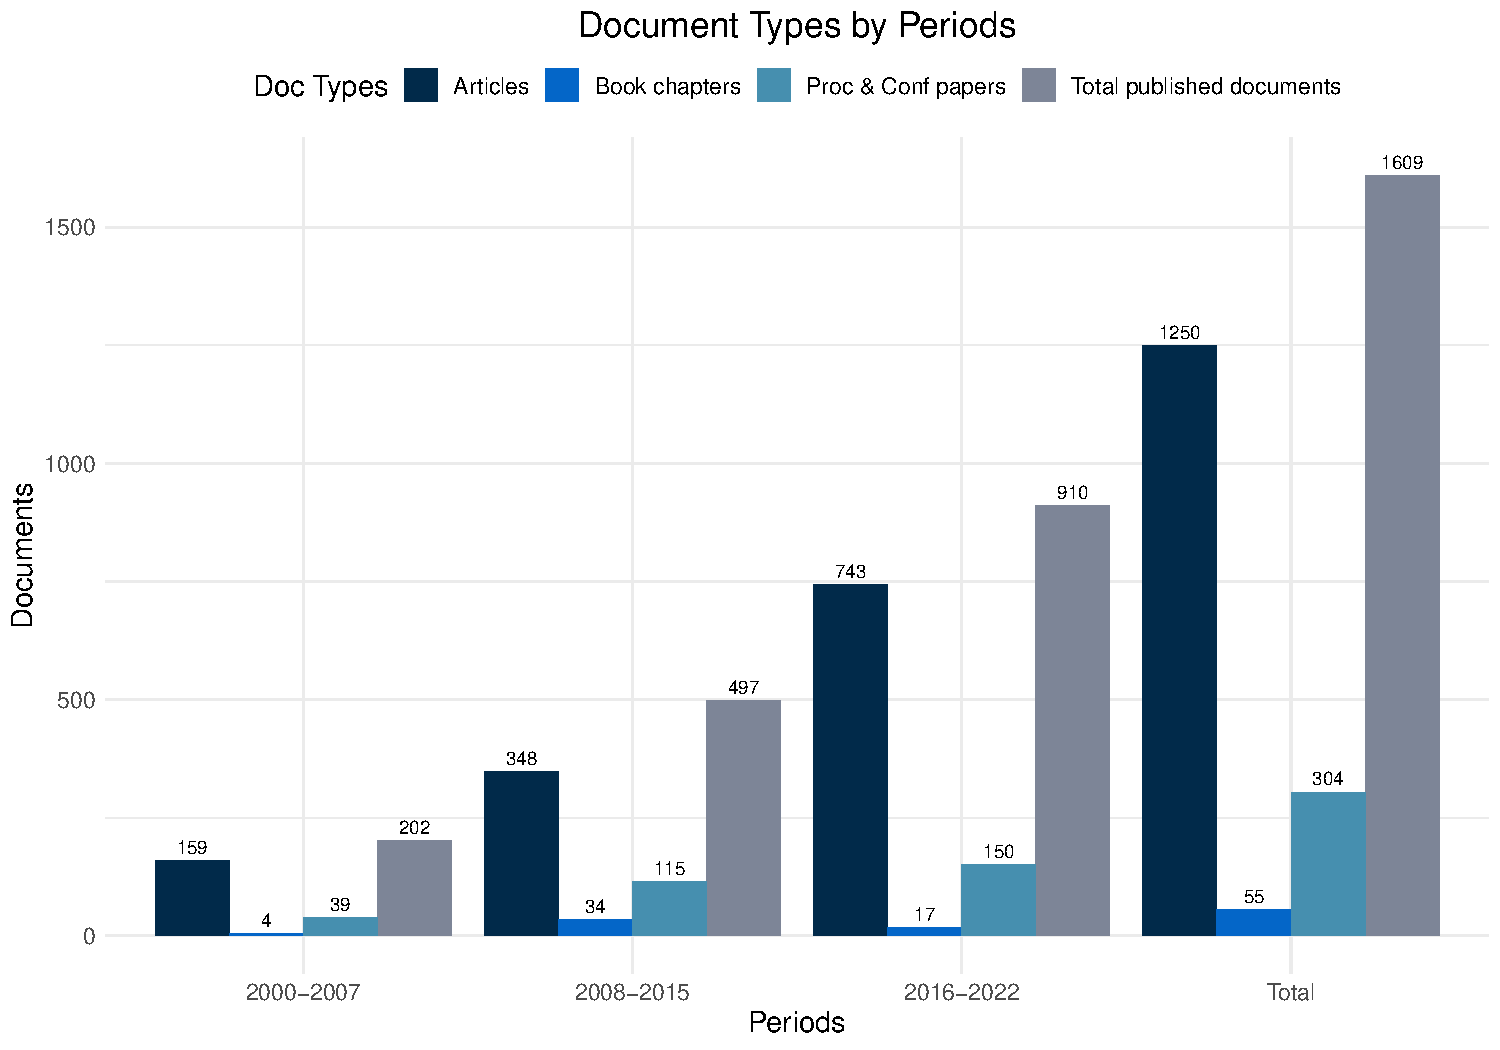
\includegraphics{Presentation_bibliometric_files/figure-beamer/doc types-1.pdf}
\end{block}
\end{frame}

\begin{frame}{6. Performance Analysis I}
\protect\hypertarget{performance-analysis-i}{}
Is a descriptive interpretation of research constituents.

\begin{block}{6.1. Publications vs Citations}
\protect\hypertarget{publications-vs-citations}{}
\vspace{0.5cm}

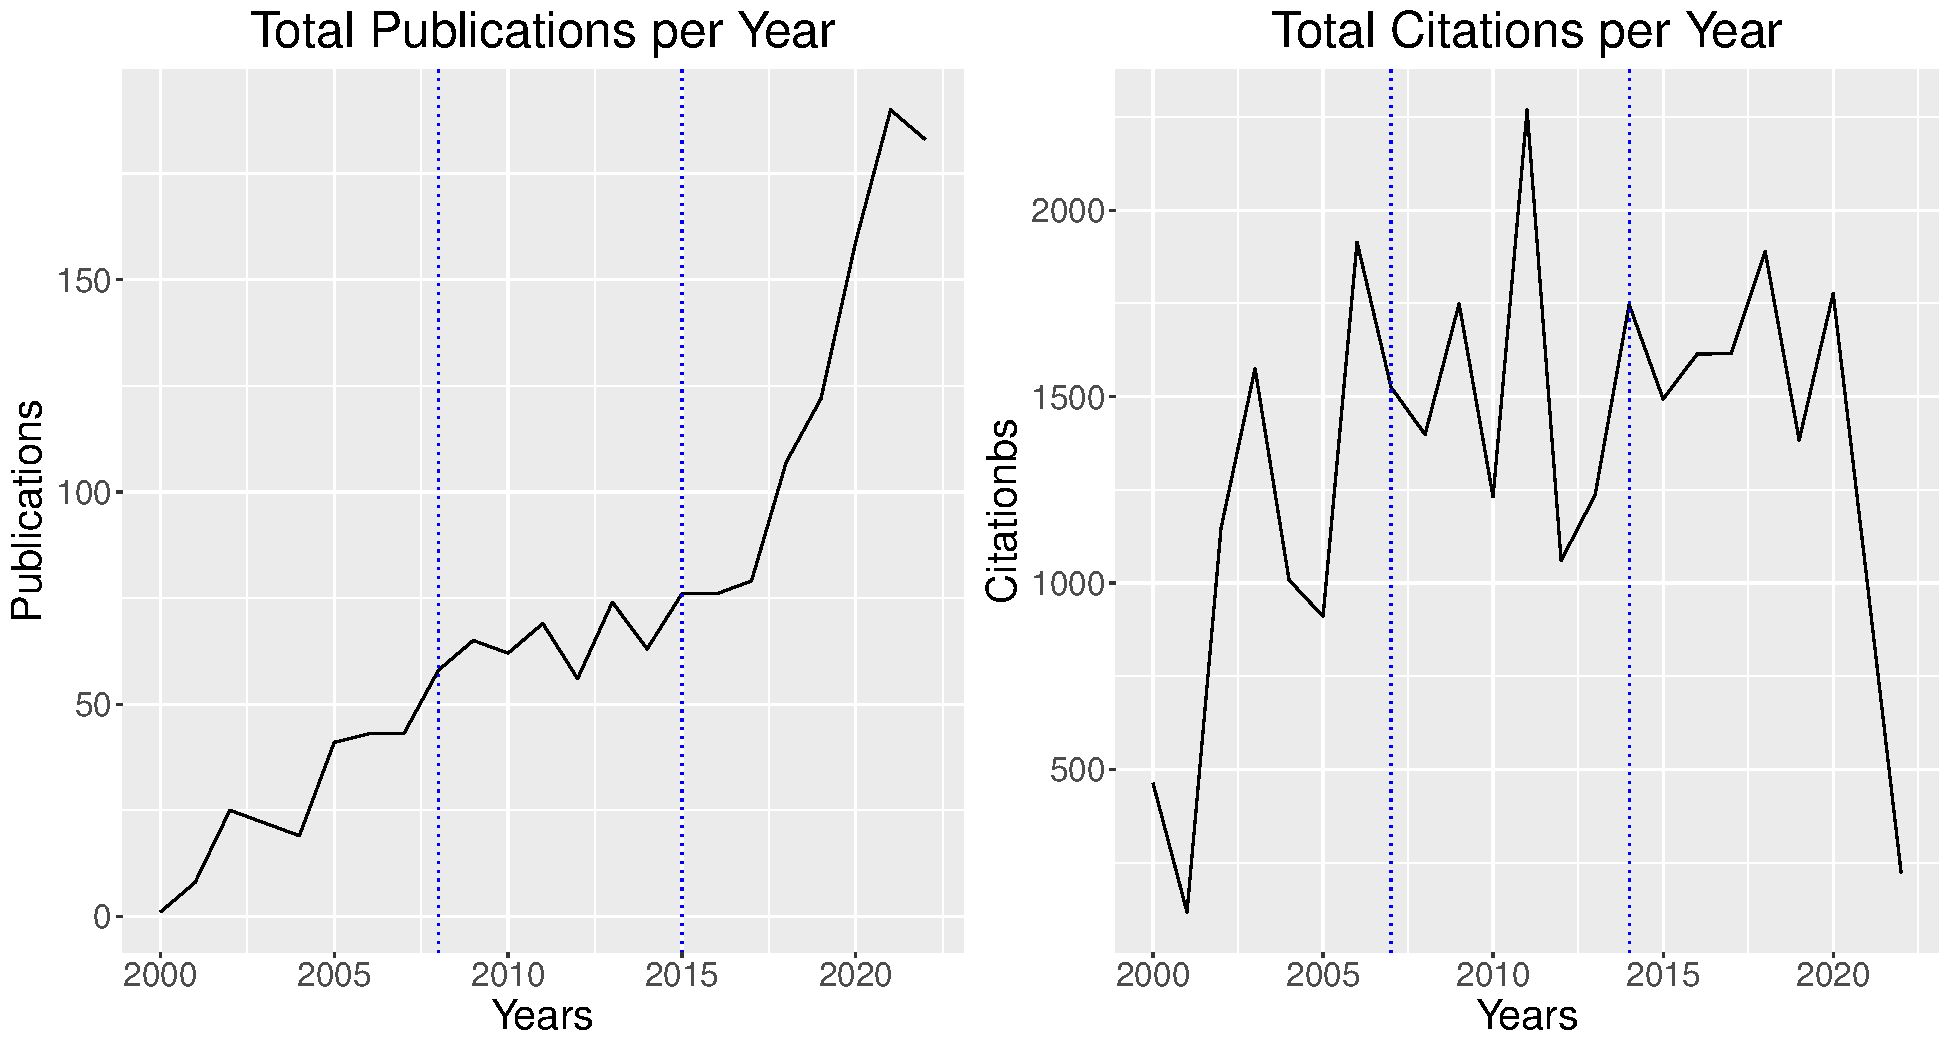
\includegraphics{Presentation_bibliometric_files/figure-beamer/Panel cite vs prod-1.pdf}
\end{block}
\end{frame}

\begin{frame}{6. Performance Analysis II}
\protect\hypertarget{performance-analysis-ii}{}
\vspace{0.5cm}

\begin{block}{6.2. Authors' publications patterns over time.}
\protect\hypertarget{authors-publications-patterns-over-time.}{}
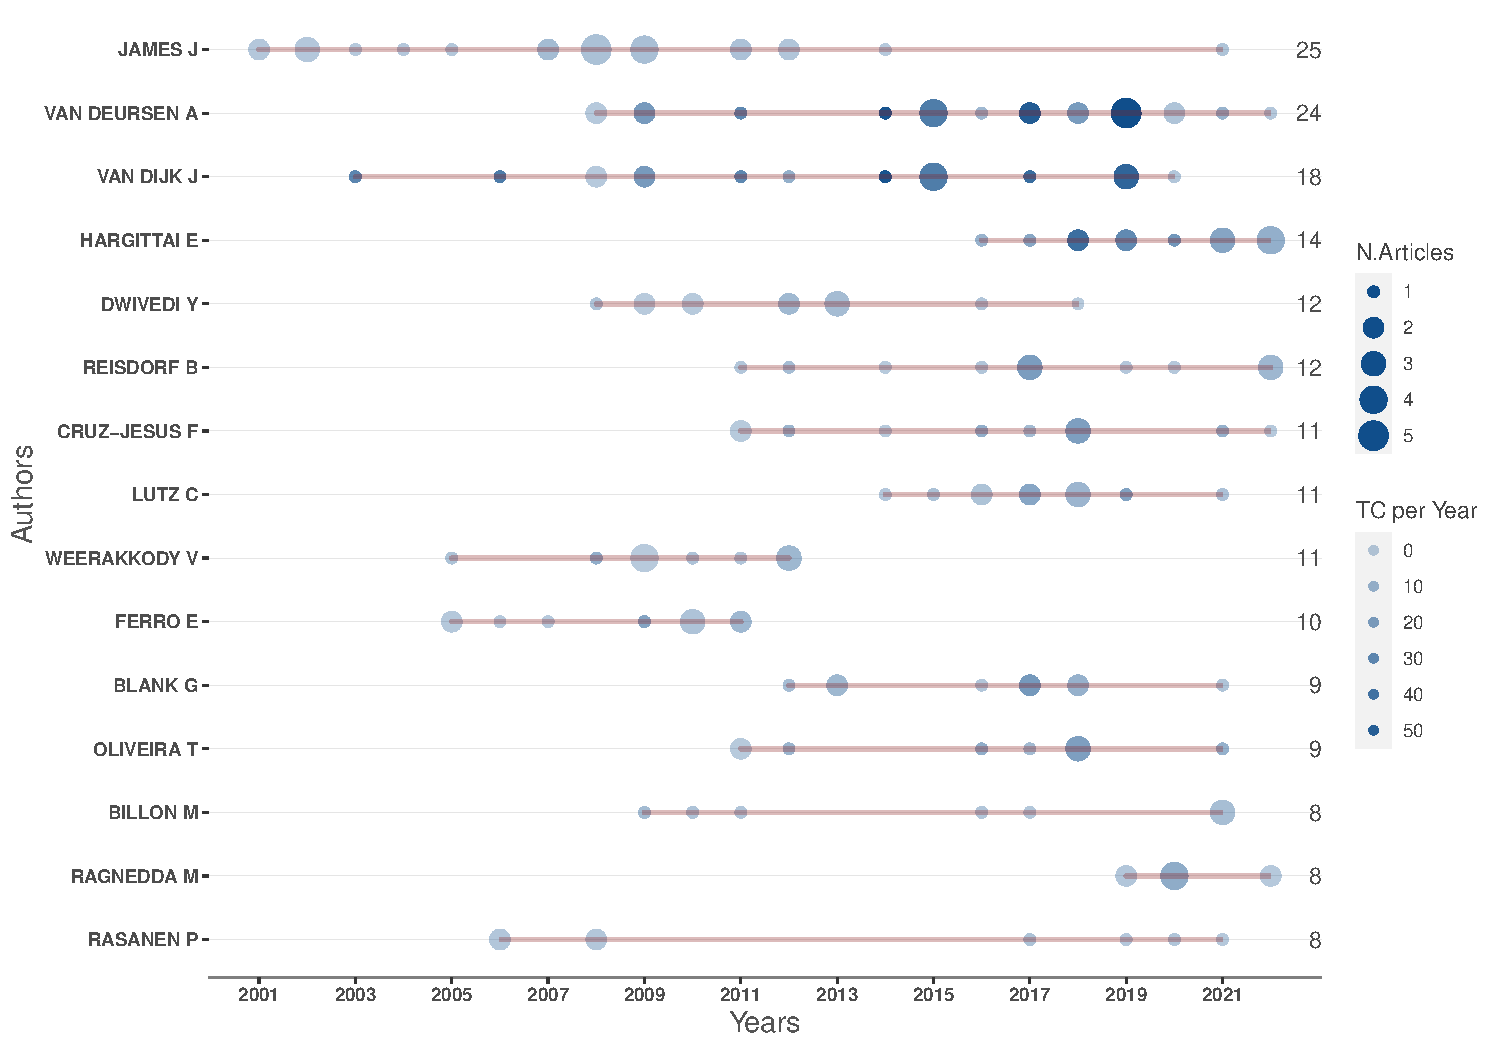
\includegraphics{Presentation_bibliometric_files/figure-beamer/Prod of AU-1.pdf}
\end{block}
\end{frame}

\begin{frame}{6. Performance Analysis III}
\protect\hypertarget{performance-analysis-iii}{}
\begin{block}{6.2. Trends in authors' citations across time periods}
\protect\hypertarget{trends-in-authors-citations-across-time-periods}{}
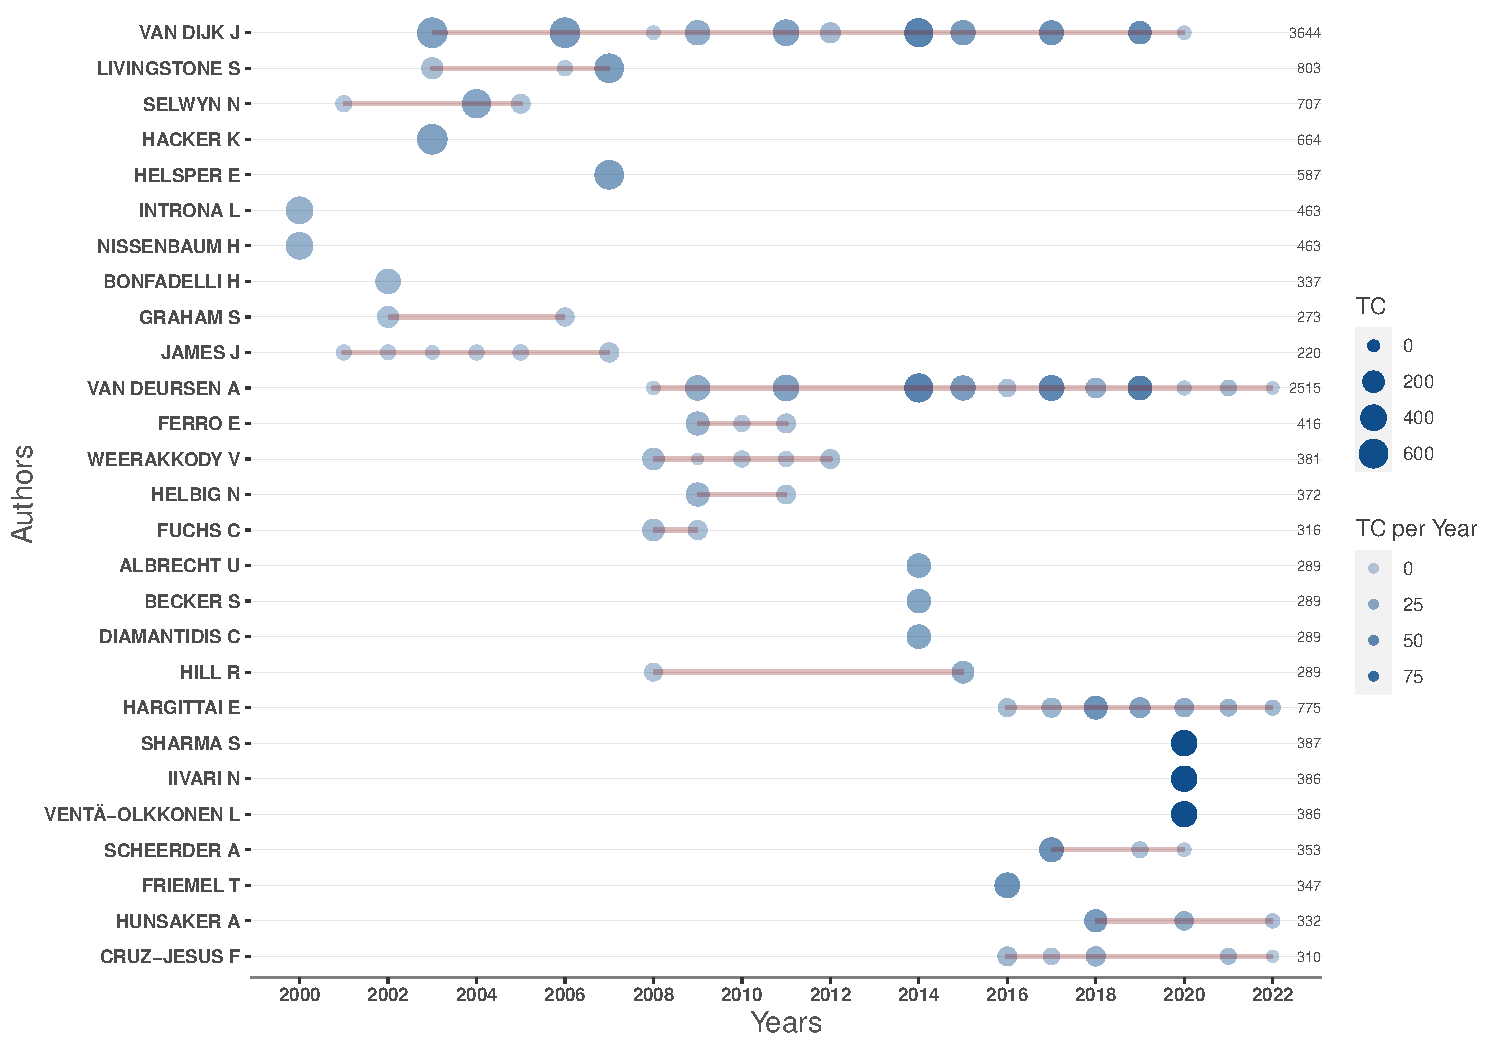
\includegraphics{Presentation_bibliometric_files/figure-beamer/Influence of AU chart-1.pdf}
\end{block}
\end{frame}

\begin{frame}{6. Performance Analysis V}
\protect\hypertarget{performance-analysis-v}{}
\begin{block}{6.2. Articles}
\protect\hypertarget{articles}{}
\begin{table}

\caption{\label{tab:Influence of AU table }Most Cited Articles}
\centering
\fontsize{5}{7}\selectfont
\begin{tabular}[t]{r|p{9cm}|r}
\hline
\textbf{Rank} & \textbf{Article} & \textbf{TC}\\
\hline
\multicolumn{3}{c}{\textbf{Period 1: 2000- 2007}}\\
\hline
\hspace{1em}1 & Van Dijk J; Hacker K (2003) -The Digital Divide As A Complex And Dynamic Phenomenon & 664\\
\hline
\hspace{1em}2 & Van Dijk J (2006) -Digital Divide Research, Achievements And Shortcomings & 660\\
\hline
\hspace{1em}3 & Livingstone S; Helsper E (2007) -Gradations In Digital Inclusion: Children, Young People And The Digital Divide & 587\\
\hline
\hspace{1em}4 & Selwyn N (2004) -Reconsidering Political And Popular Understandings Of The Digital Divide & 560\\
\hline
\hspace{1em}5 & Introna L; Nissenbaum H (2000) -Shaping The Web: Why The Politics Of Search Engines Matters & 463\\
\hline
\multicolumn{3}{c}{\textbf{Period 2: 2008- 2015}}\\
\hline
\hspace{1em}1 & Van Deursen A; Van Dijk J (2014) -The Digital Divide Shifts To Differences In Usage & 555\\
\hline
\hspace{1em}2 & Van Deursen A; Van Dijk J (2011) -Internet Skills And The Digital Divide & 402\\
\hline
\hspace{1em}3 & Becker S; Miron-Shatz T; Schumacher N; Krocza J; Diamantidis C; Albrecht U (2014) -Mhealth 2.0: Experiences, Possibilities, And Perspectives & 289\\
\hline
\hspace{1em}4 & Helbig N; Gil-García J; Ferro E (2009) -Understanding The Complexity Of Electronic Government: Implications From The Digital Divide Literature & 268\\
\hline
\hspace{1em}5 & Carter L; Weerakkody V (2008) -E-Government Adoption: A Cultural Comparison & 208\\
\hline
\multicolumn{3}{c}{\textbf{Period 3: 2016- 2022}}\\
\hline
\hspace{1em}1 & Iivari N; Sharma S; Ventä-Olkkonen L (2020) -Digital Transformation Of Everyday Life – How Covid-19 Pandemic Transformed The Basic Education Of The Young Generation And Why Information Management Research Should Care? & 386\\
\hline
\hspace{1em}2 & Friemel T (2016) -The Digital Divide Has Grown Old: Determinants Of A Digital Divide Among Seniors & 347\\
\hline
\hspace{1em}3 & Scheerder A; Van Deursen A; Van Dijk J (2017) -Determinants Of Internet Skills, Uses And Outcomes. A Systematic Review Of The Second- And Third-Level Digital Divide & 307\\
\hline
\hspace{1em}4 & Hunsaker A; Hargittai E (2018) -A Review Of Internet Use Among Older Adults & 223\\
\hline
\hspace{1em}5 & Van Deursen A; Van Dijk J (2019) -The First-Level Digital Divide Shifts From Inequalities In Physical Access To Inequalities In Material Access & 198\\
\hline
\multicolumn{3}{l}{\textsuperscript{1} Source: Author's elaboration}\\
\multicolumn{3}{l}{\textsuperscript{2} TC: Times Cited}\\
\end{tabular}
\end{table}
\end{block}
\end{frame}

\begin{frame}{6. Performance Analysis VI}
\protect\hypertarget{performance-analysis-vi}{}
\begin{block}{6.3. Journals}
\protect\hypertarget{journals}{}
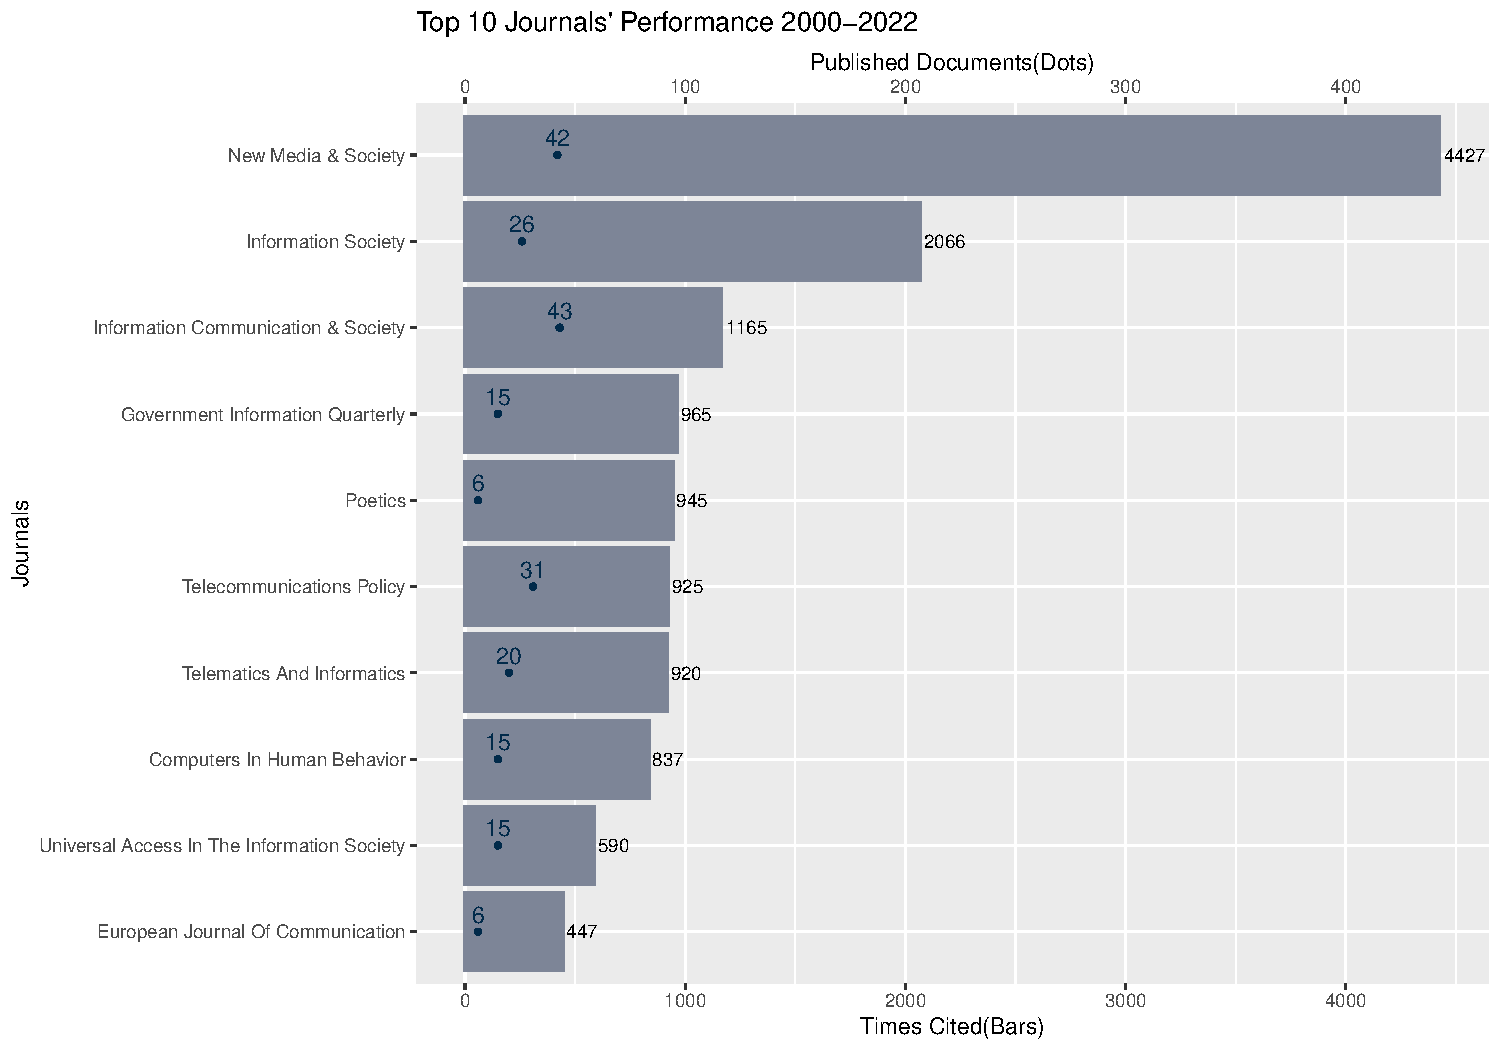
\includegraphics{Presentation_bibliometric_files/figure-beamer/Influencial SO-1.pdf}
\end{block}
\end{frame}

\begin{frame}{6. Performance Analysis VII}
\protect\hypertarget{performance-analysis-vii}{}
\begin{block}{6.4. Affiliations/ Universities}
\protect\hypertarget{affiliations-universities}{}
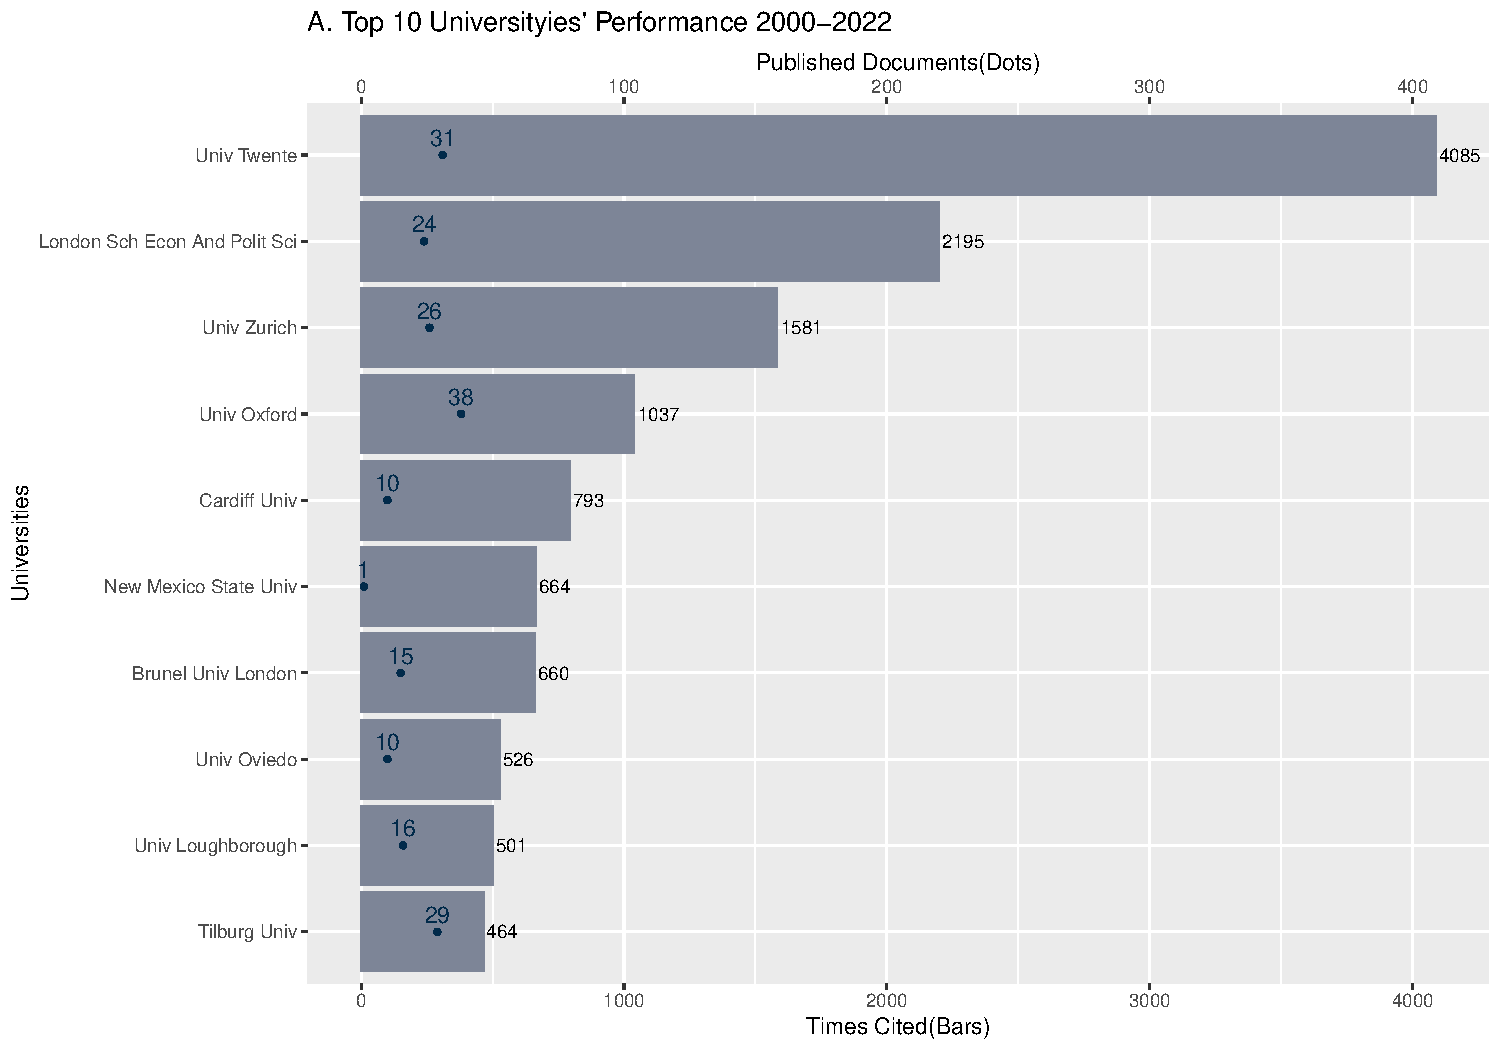
\includegraphics{Presentation_bibliometric_files/figure-beamer/Influencial UN-1.pdf}
\end{block}
\end{frame}

\begin{frame}{6. Performance Analysis VIII}
\protect\hypertarget{performance-analysis-viii}{}
\begin{block}{6.5. Countrys' Performance 2000-2022}
\protect\hypertarget{countrys-performance-2000-2022}{}
\vspace{0.5cm}

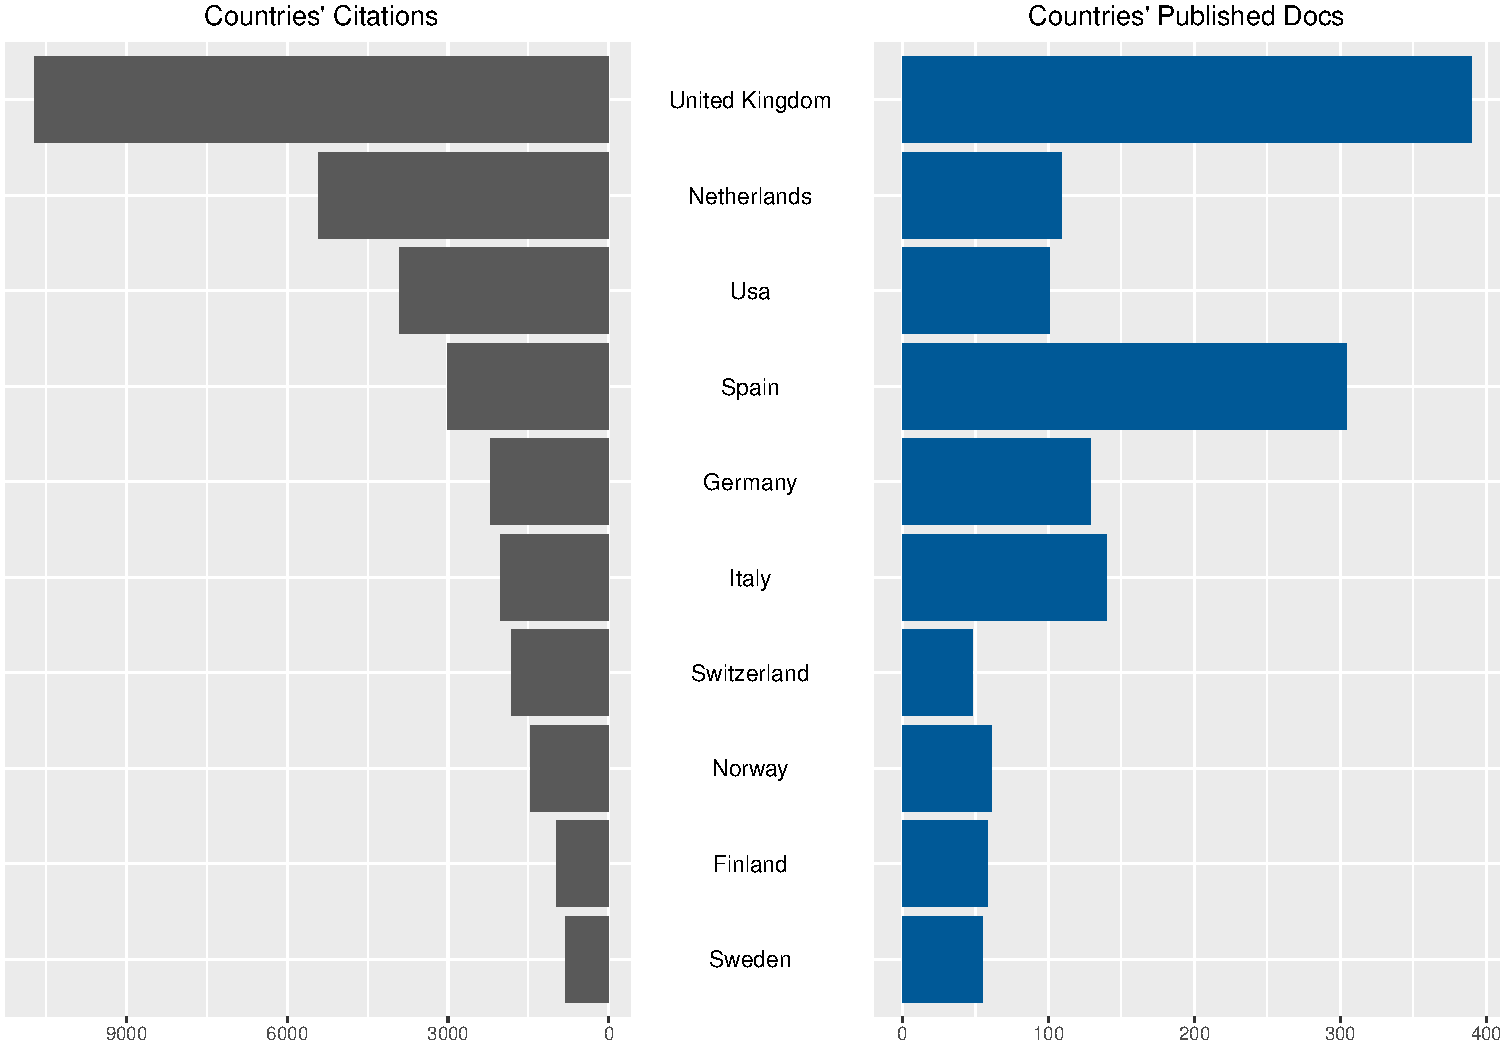
\includegraphics{Presentation_bibliometric_files/figure-beamer/Influencial CO-1.pdf}
\end{block}
\end{frame}

\begin{frame}{6. Performance Analysis IX}
\protect\hypertarget{performance-analysis-ix}{}
\begin{block}{6.6. Countries Collaboration Network}
\protect\hypertarget{countries-collaboration-network}{}
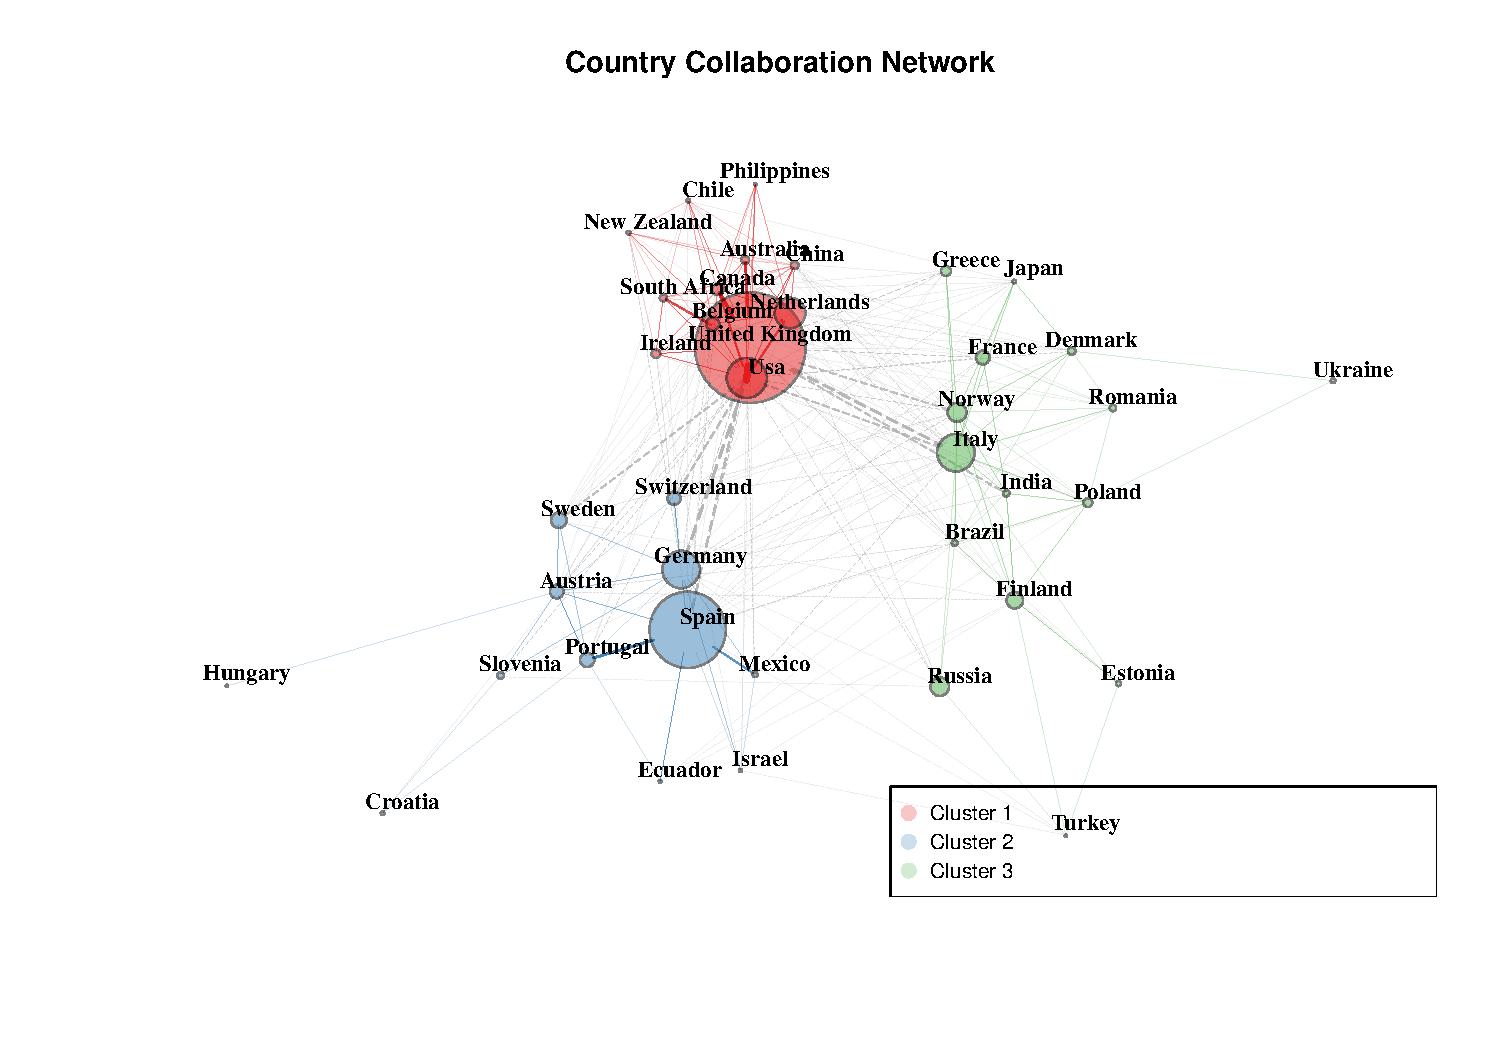
\includegraphics{Presentation_bibliometric_files/figure-beamer/Network CO-1.pdf}
\end{block}
\end{frame}

\begin{frame}{7. Science Mapping I}
\protect\hypertarget{science-mapping-i}{}
Is a set of techniques and tools used to visualize and analyze the
structure, relationships, and patterns within a scientific field or
discipline.

\begin{block}{7.1. Citation Analysis}
\protect\hypertarget{citation-analysis}{}
\begin{table}[!h]

\caption{\label{tab:Most cited refs}Most Cited References 2000-2022}
\centering
\fontsize{5}{7}\selectfont
\begin{tabular}[t]{r|p{9cm}|r}
\hline
\textbf{Rank} & \textbf{Article} & \textbf{TC}\\
\hline
1 & Norris P (2001) -Digital Divide Civic Engagement, Information Poverty, And The Internet Worldwide & 204\\
\hline
2 & Van Dijk J (2005) -The Deepening Divide: Inequality In The Information Society & 172\\
\hline
3 & Hargittai E (2002) -Second-Level Digital Divide: Differences In People's Online Skills & 136\\
\hline
4 & Van Dijk J (2006) -Digital Divide Research, Achievements And Shortcomings & 129\\
\hline
5 & Van Dijk J, Hacker K (2003) -The Digital Divide As A Complex And Dynamic Phenomenon & 114\\
\hline
6 & Selwyn N (2004) -Reconsidering Political And Popular Understandings Of The Digital Divide & 108\\
\hline
7 & Dimaggio P, Hargittai E, Celeste C, Shafer S (2004) -From Unequal Access To Differentiated Use: A Literature Review And Agenda For Research On Digital Inequality & 105\\
\hline
8 & Van Deursen A, Van Dijk J (2014) -The Digital Divide Shifts To Differences In Usage & 103\\
\hline
9 & Zillien N, Hargittai E (2009) -Digital Distinction: Status-Specific Types Of Internet Usage & 82\\
\hline
10 & Hargittai E, Hinnant A (2008) -Digital Inequality: Differences In Young Adults' Use Of The Internet & 80\\
\hline
\multicolumn{3}{l}{\textsuperscript{1} Source: Author's elaboration}\\
\multicolumn{3}{l}{\textsuperscript{2} TC: Times Cited}\\
\end{tabular}
\end{table}
\end{block}
\end{frame}

\begin{frame}{7. Science Mapping II}
\protect\hypertarget{science-mapping-ii}{}
\begin{block}{7.2. Similarity measures}
\protect\hypertarget{similarity-measures}{}
Quantify similarity, connections and relationships among academic
entities.

Following \citet{kammerer2021}

\begin{itemize}
\item
  \textbf{Knowledge base:} cluster of academic publications in a
  research field that are considered fundamental to the development and
  understanding of the field.
\item
  \textbf{Research front:} cluster of academic publications that refers
  to emerging active areas of research considering themselves with a
  similar unsolved research problem.
\end{itemize}

\begin{center}
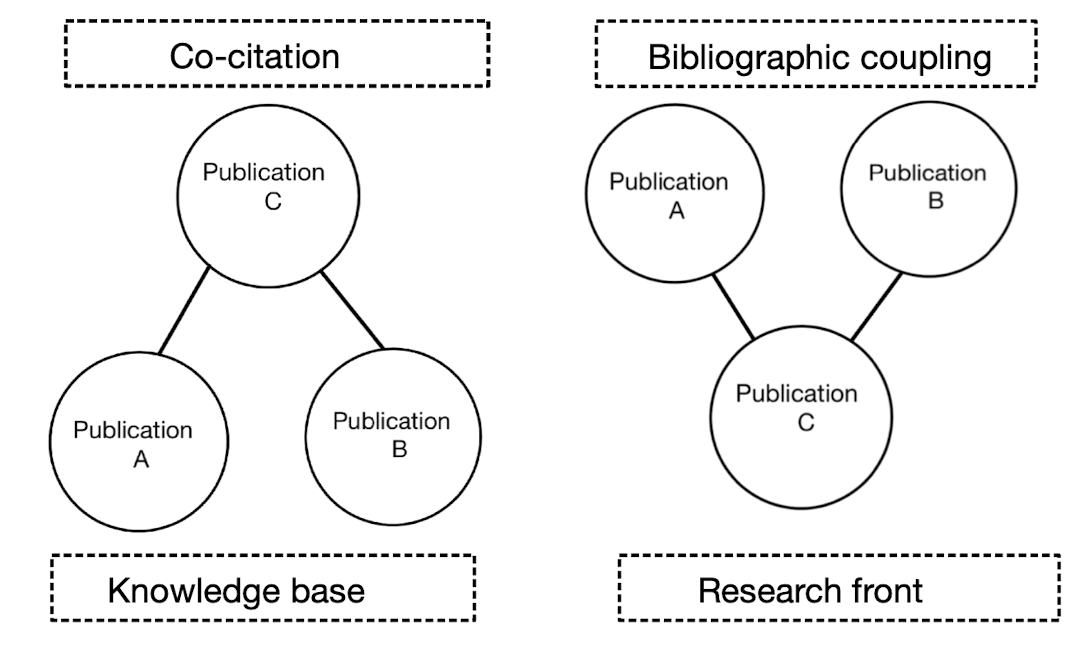
\includegraphics[width=0.6\textwidth]{pic_1.png}
\end{center}
\end{block}
\end{frame}

\begin{frame}{7. Science Mapping III}
\protect\hypertarget{science-mapping-iii}{}
\vspace{0.5cm}

\begin{block}{7.2.1. Co-citations Analyisis}
\protect\hypertarget{co-citations-analyisis}{}
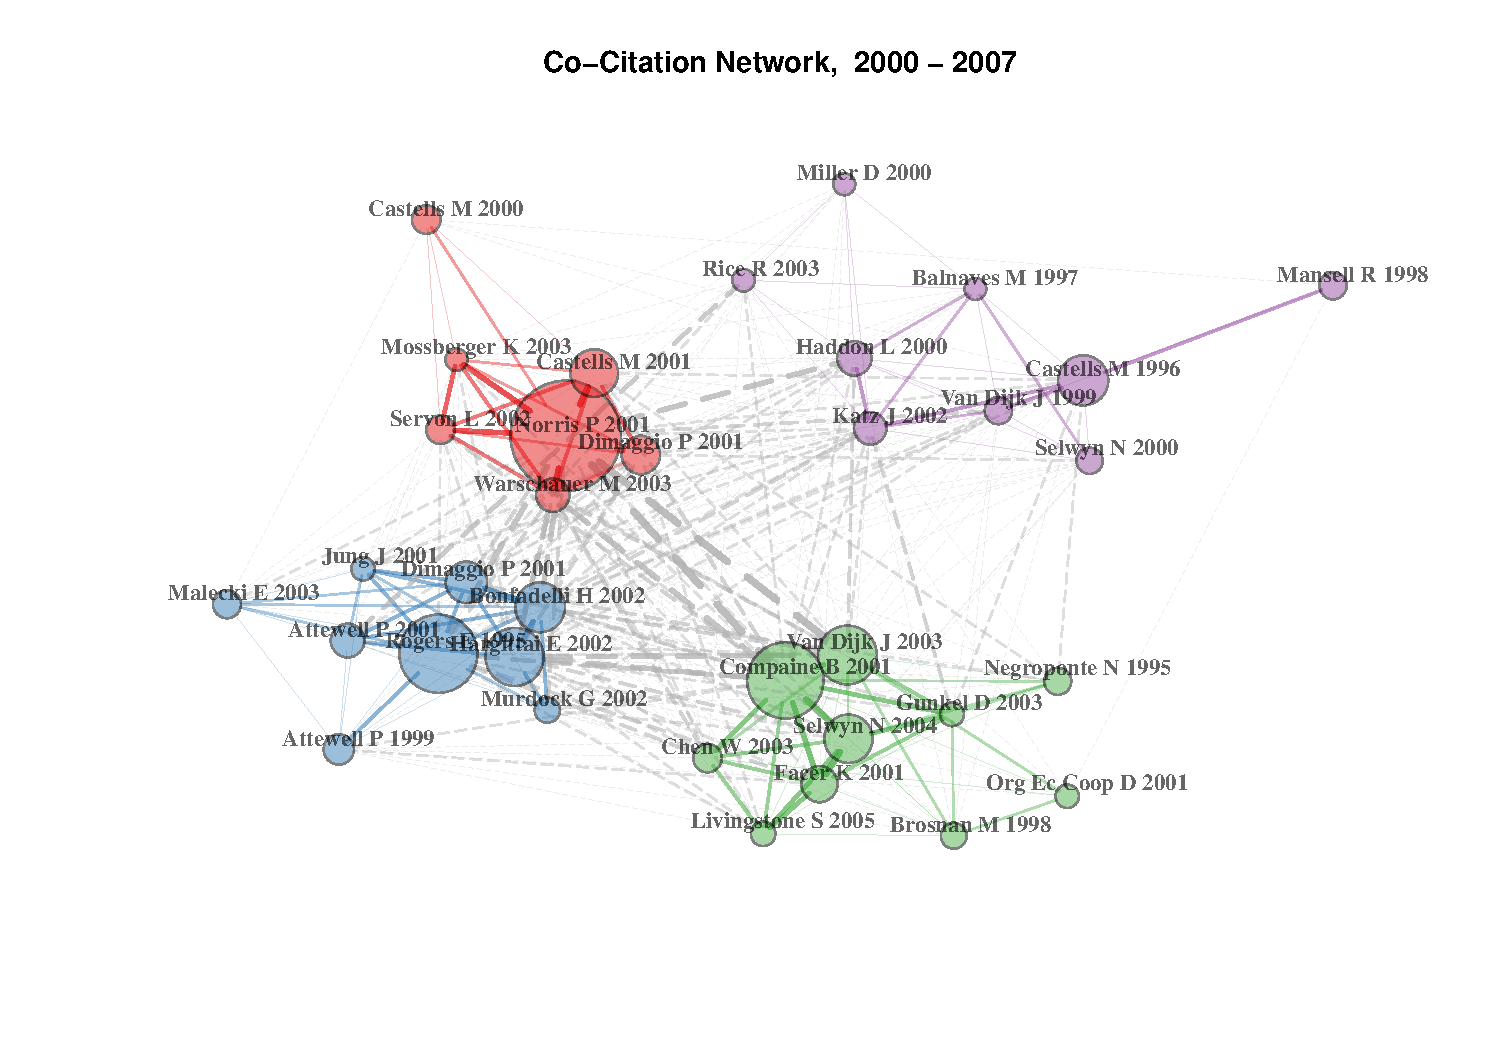
\includegraphics{Presentation_bibliometric_files/figure-beamer/Co_cite_P1-1.pdf}
\end{block}
\end{frame}

\begin{frame}{7. Science Mapping IV}
\protect\hypertarget{science-mapping-iv}{}
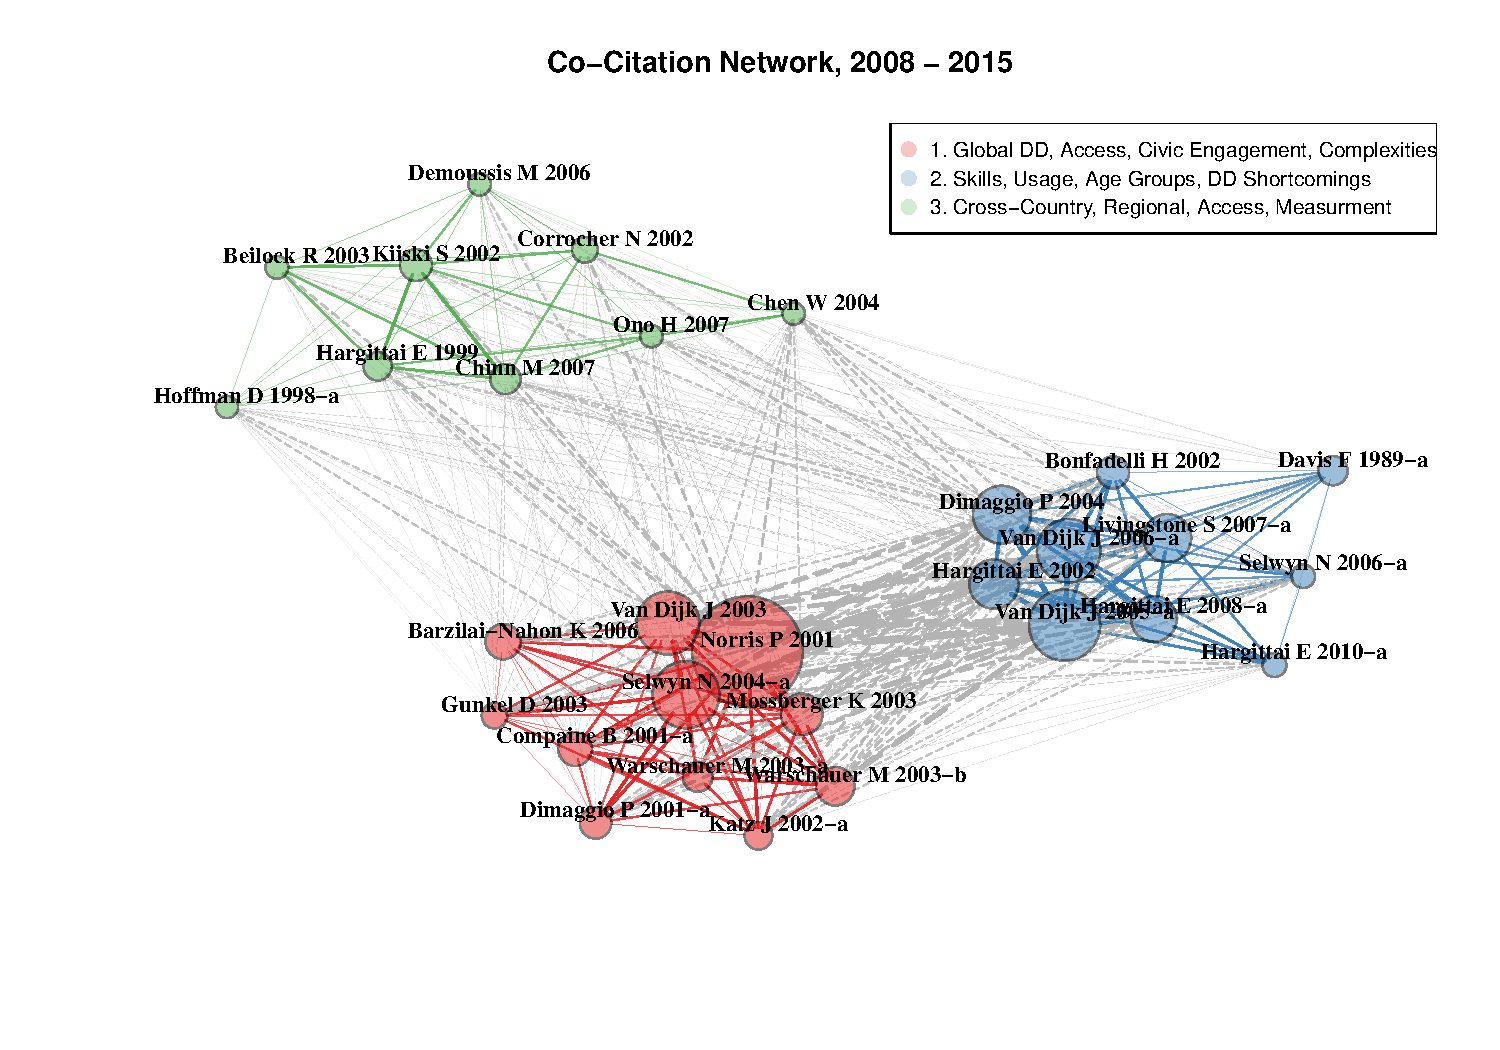
\includegraphics{Presentation_bibliometric_files/figure-beamer/Co_cite_P2-1.pdf}
\end{frame}

\begin{frame}{7. Science Mapping V}
\protect\hypertarget{science-mapping-v}{}
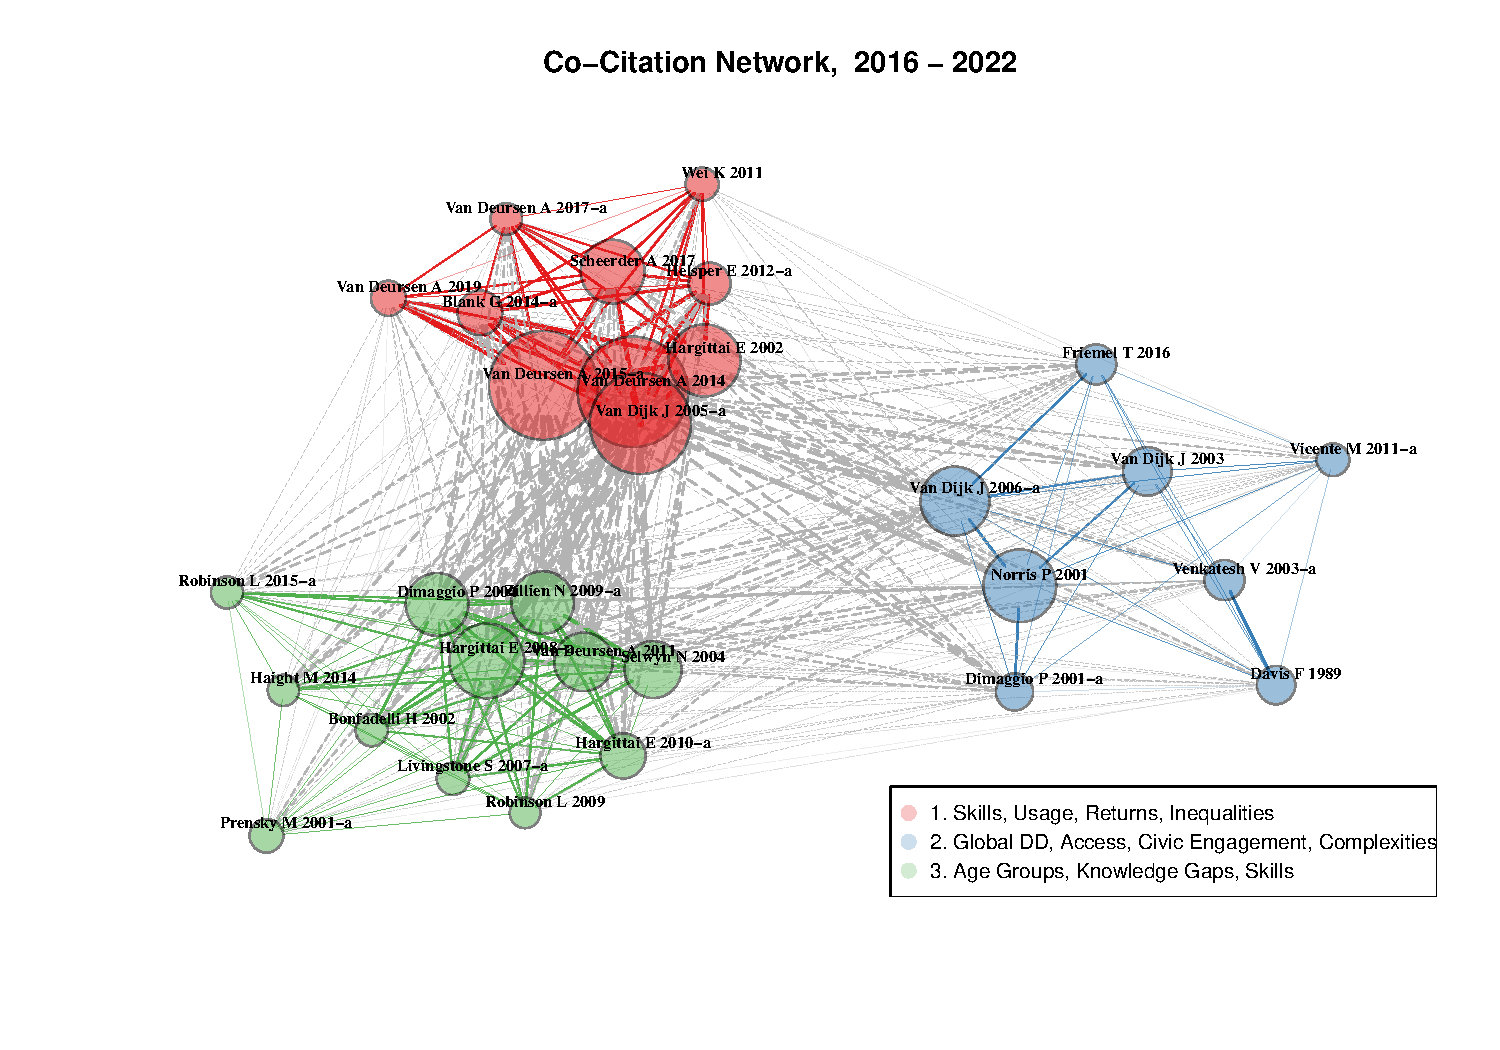
\includegraphics{Presentation_bibliometric_files/figure-beamer/Co_cite_P3-1.pdf}
\end{frame}

\begin{frame}{7. Science Mapping VI}
\protect\hypertarget{science-mapping-vi}{}
\begin{block}{Co-citation Networks Summary}
\protect\hypertarget{co-citation-networks-summary}{}
This three networks highlighted:

\begin{itemize}
\item
  \textbf{Evolution of research focus:} From internet access and
  infrastructure to the various facets of the digital divide.
\item
  \textbf{Key authors and publications:} These form the knowledge
  foundations that shapes the discourse, broaden the comprehension of
  the literature, and guide future research.
\item
  \textbf{Emerging trends and themes:} These networks have assisted in
  uncovering growing themes that highlight research directions that
  require further examination.
\end{itemize}
\end{block}
\end{frame}

\begin{frame}{7. Science Mapping VII}
\protect\hypertarget{science-mapping-vii}{}
\begin{block}{7.2.2. Bibliographic Coupling Analysis}
\protect\hypertarget{bibliographic-coupling-analysis}{}
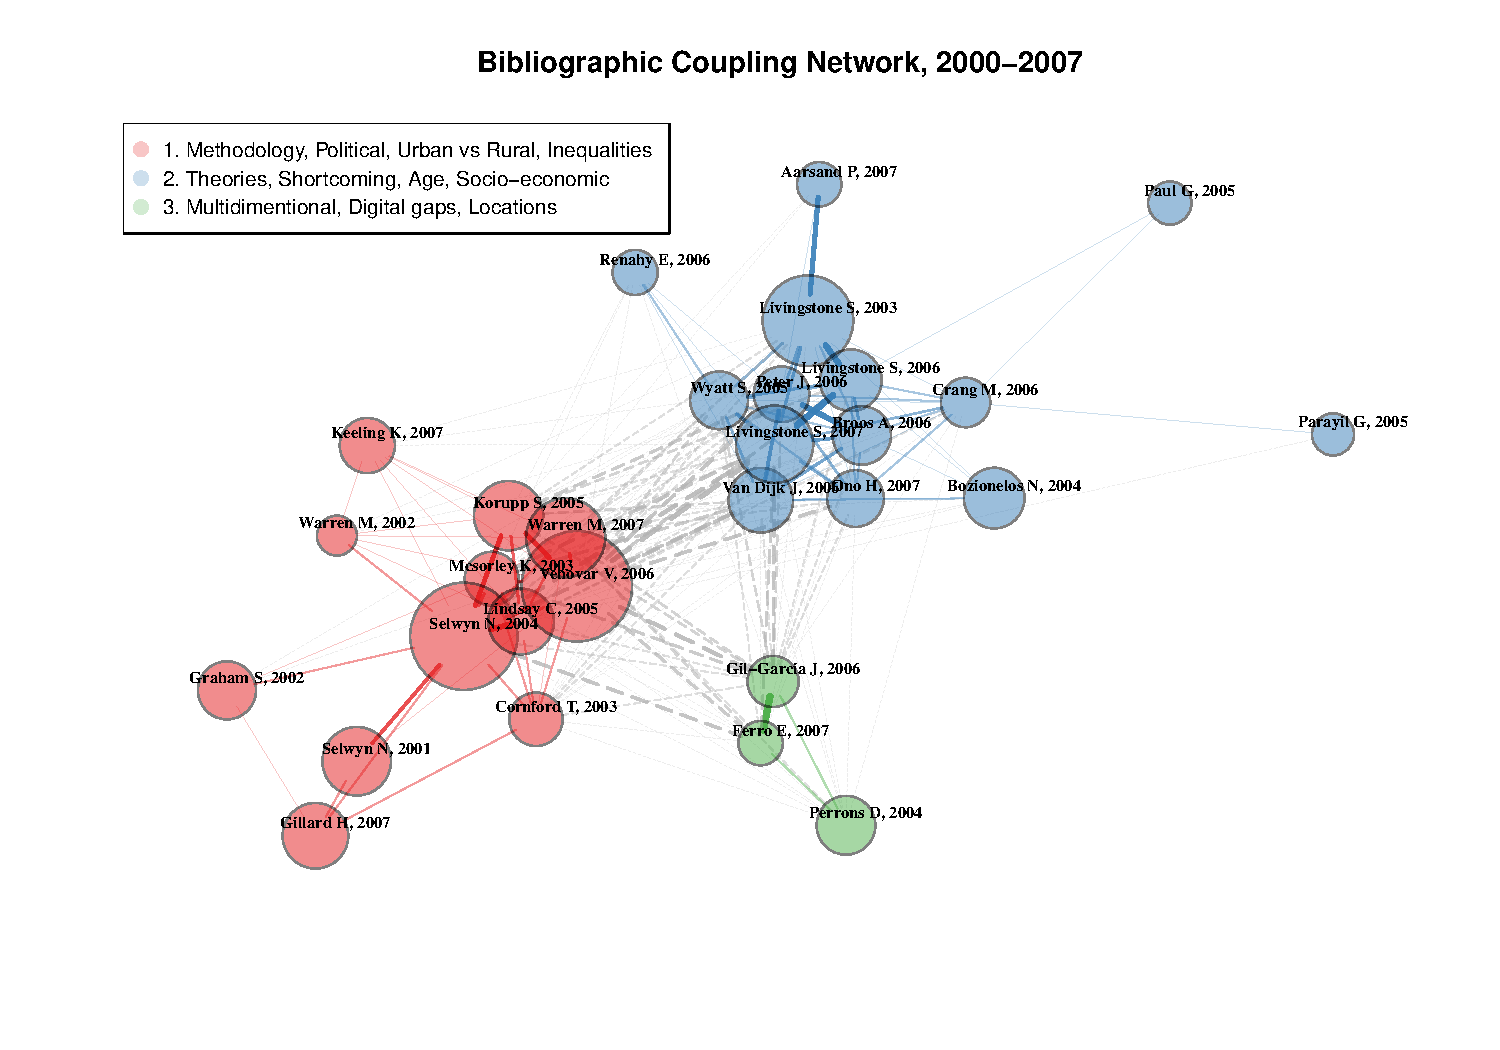
\includegraphics{Presentation_bibliometric_files/figure-beamer/Bib_coup_P1-1.pdf}
\end{block}
\end{frame}

\begin{frame}{7. Science Mapping VIII}
\protect\hypertarget{science-mapping-viii}{}
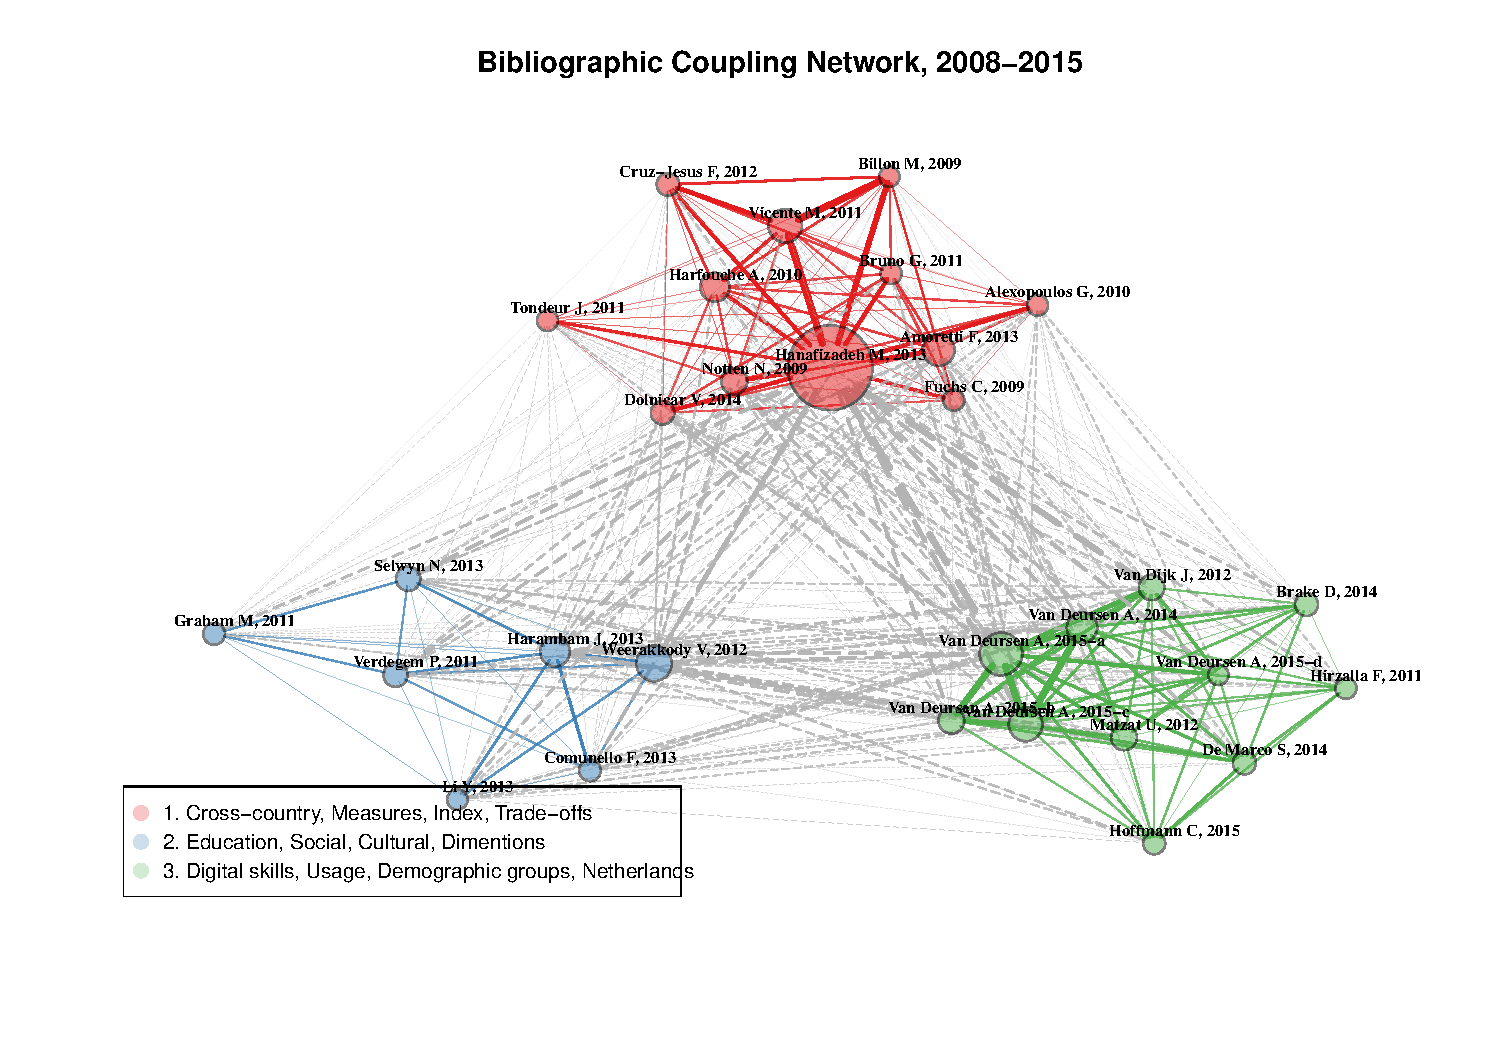
\includegraphics{Presentation_bibliometric_files/figure-beamer/Bib_coup_P2-1.pdf}
\end{frame}

\begin{frame}{7. Science Mapping IX}
\protect\hypertarget{science-mapping-ix}{}
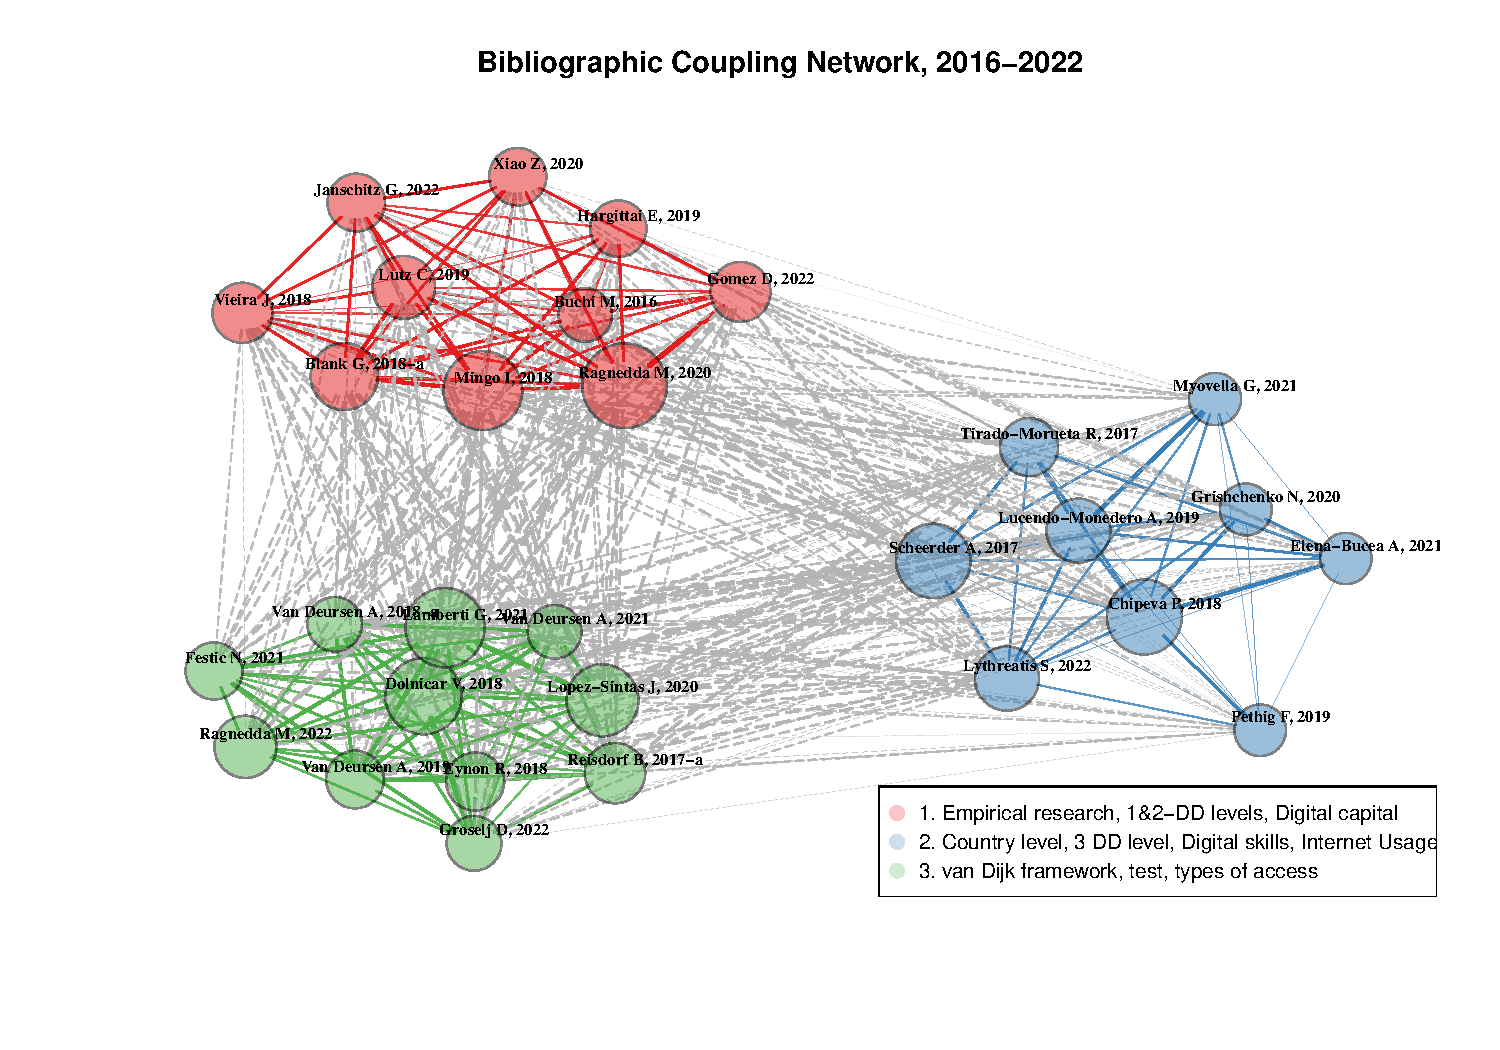
\includegraphics{Presentation_bibliometric_files/figure-beamer/Bib_coup_P3-1.pdf}
\end{frame}

\begin{frame}{7. Science Mapping X}
\protect\hypertarget{science-mapping-x}{}
\begin{block}{Bibliographic coupling Networks Summary}
\protect\hypertarget{bibliographic-coupling-networks-summary}{}
This three networks highlighted:

\begin{itemize}
\item
  \textbf{Evolution of digital divide research:} Themes move from access
  and socio-demographic factors to a more nuance understanding of
  skills, usage and emerging technologies.
\item
  \textbf{Emergence of key authors:} Represent the influential authors
  that contributed in the emergence of active areas of research in the
  development of the digital divide.
\item
  \textbf{Growing complexities and specialization:} The diverse research
  themes in the networks reflect the expanding scope and depth of
  digital divide research.
\end{itemize}
\end{block}
\end{frame}

\begin{frame}{7. Science Mapping XI}
\protect\hypertarget{science-mapping-xi}{}
\begin{block}{7.2.2. Co-word Analysis}
\protect\hypertarget{co-word-analysis}{}
\end{block}
\end{frame}

\begin{frame}{Conclusions}
\protect\hypertarget{conclusions}{}
\begin{itemize}
\item
  We have seen the main trends and focus shifts: from access,
  infrastructure, and socio-economic factors, to skills, usage and other
  facets of the digital divide, this highlights the complexity and
  multidimensionality of the digital divide.
\item
  The networks showcase collaboration among prominent authors that
  consistently contribute in the field. The thematic relationships show
  interconnections of various aspects of the digital divide.
\item
  European studies have not extensively addressed the corporate digital
  divide, leaving room for further examination. The corporate digital
  divide might be incorporated into other literature streams, such as
  digital transformation and technology adoption.
\end{itemize}
\end{frame}

\begin{frame}{Contact information}
\protect\hypertarget{contact-information}{}
\vspace{2cm}

Luis Carlos Castillo-Tellez

\vspace{0.1cm}

Guest Researcher

PhD candidate in Global Studies

University of Urbino - Italy

email:
\href{mailto:l.castillotellez@campus.uniurb.it}{\nolinkurl{l.castillotellez@campus.uniurb.it}}

email:
\href{mailto:luiscarl@uni-bremen.de}{\nolinkurl{luiscarl@uni-bremen.de}}
\end{frame}

\renewcommand\refname{References}
\begin{frame}[allowframebreaks]{References}
  \bibliographytrue
  \bibliography{references.bib}
\end{frame}

\end{document}
